\documentclass[12pt]{article}

\usepackage{sbc-template}

\usepackage{graphicx,url}

%\usepackage[brazil]{babel}   
\usepackage[utf8]{inputenc}  

     
\sloppy

\title{Projeto de Programação}

\author{Diego O. Lemos\inst{1}, Gildo A. S. Freitas\inst{1}, Jeferson F. Ribeiro\inst{1},\\
Joaliton L. P. Ferreira\inst{1} Pedro H. R. Emerick\inst{1}, Valmir C. S. Junior\inst{1} }

\address{Instituto Metrópole Digital -- Universidade Federal do Rio Grande do Norte
  (UFRN)\\Natal -- RN -- Brazil
  \email{\{diegoifrn,gildo.augu,jfrsnr\}@gmail.com}
  \email{p.emerick@live.com, \{luanpereira00,valmircorrea96\}@outlook.com}
}

\begin{document} 

\maketitle

\begin{abstract}
This article refers to a project developed in computer networking course in the second semester of 2017, taught by the professor Wellington Silva de Souza at Federal University of Rio Grande do Norte (UFRN). This project had both exploratory and educative natures, and its aim was to implement a NTP (Network Time Protocol) server using RPi (Raspberry Pi) and a GPS (Global Positioning System) clock adapter.
\end{abstract}
     
\begin{resumo} 
Este artigo é referente a um trabalho desenvolvido na disciplina de Redes de Computadores, ministrada pelo Professor Wellington Silva De Souza na Universidade Federal do Rio Grande do Norte (UFRN), no segundo semestre do ano de 2017. O trabalho foi desenvolvido com cunho exploratório e educativo para demonstrar como implementar um servidor \textit{NTP (Network Time Protocol}) usando \textit{RPi (Raspberry Pi)} e uma fonte de relógio \textit{GPS (Global Positioning System)}.
\end{resumo}


\section{Introdução}

O \textit{NTP (Network Time Protocol)} pertence à camada de aplicação e tem como objetivo sincronizar os relógios de computadores. Baseado no protocolo \textit{UDP (User Datagram Protocol)} sob a porta 123, o uso do NTP permite manter o relógio de um computador com a hora sempre certa e com exatidão. 

O protocolo funciona baseado na troca de mensagens entre cliente e servidor, onde o cliente faz a leitura de seu relógio e envia ao servidor em forma de mensagem o resultado. O servidor recebe a mensagem e realiza a leitura do seu relógio próprio, e, mantêm as duas informações.
Após um período de tempo o servidor realiza a leitura de seu relógio novamente e envia ao cliente uma mensagem com as três informações (tempo recebido do cliente, tempo inicial próprio e tempo final próprio). Após receber essa mensagem o cliente envia um novo tempo para o servidor, sendo esse o seu tempo final. O protocolo executa várias trocas de mensagens como as descritas acima, e, utilizando o algoritmo de filtro de relógio para escolher os pares de informações da mensagem mais condizente com a realidade, o algoritmo de seleção de relógio para escolher os confiáveis entre os filtrados.

Partindo disso, o objetivo desse trabalho foi implementar um servidor NTP. Para a execução do projeto foi necessário utilizar um computador para dar suporte ao sistema NTP e um módulo de GPS para obter sinais de GPS via satélite.

\section{Revisão da Literatura}
A presente seção tem por finalidade explicitar sucintamente alguns conceitos que serão discutidos durante a instalação e configuração (video Anexo 1) do servidor NTP no Raspberry Pi, que é um computador de baixo custo e com um tamanho muito menor que os computadores tradicionais \cite{foundation}.

A escolha pelo Raspberry Pi se justifica por ele ser um computador compacto e eficiente \cite{nayyar}. O Raspberry Pi suporta diversas linguagens de programação assim como diversos sistemas operacionais, pois opera como open source. A placa também possui muitas entradas e saídas que foram essenciais para execução do experimento.

O NTP é descrito pelo sítio NTP.BR \cite{ntp-br} como o Protocolo de Tempo para Redes (Network Time Protocol, em inglês) e é o protocolo responsável por permitir sincronização de relógio entre dispositivos conectados à rede através de referências de tempo confiáveis. 

A referência de tempo é confiável quando ela está de acordo com um relógio atômico de césio que, segundo \cite{tuboy}, a unidade de tempo (segundo) medido por este relógio atômico é a medida física mais bem definida. Ainda segundo \cite{tuboy}, servidores NTP também são comumente implementados com requisições de sinais de satélite. 

O uso de relógios atômicos em satélites para uso do sistema de posicionamento global (GPS) é extremamente necessário, pois, o tempo é utilizado para identificar a localização do receptor, com margem de erro de poucos metros [Tuboy et al., s.d.]. A forma para determinar o posicionamento comumente usada é através de um GPS autônomo que calcula órbitas de satélite GPS e pseudo-distâncias para os satélites (triangulação de no mínimo 3 satélites) usando um chipset ou módulo GPS montado em um circuito terminal e que determina a localização do terminal do objeto \cite{Jeon}. OS GPSs atuais costumam usar o sinal PPS (Pulse Per Second) no intuito de obter uma performance ainda melhor no que se refere a construção do servidor NTP\cite{corcoran}.
 
Os servidores NTP possuem uma topologia em camadas, cada qual chamada de Stratum. O Stratum 0  geralmente é um GPS ou um relógio atômico. O Stratum 1 representa os computadores que se anexam aos dispositivos de Stratum 0 para atuarem como servidores para os dispositivos de Stratum 2. Computadores de Stratum 2 normalmente mandam requisições NTP para mais de um servidor, assim como paream com outros computadores de Stratum 2 com objetivo de produzir robustez e estabilidade no tempo. Do Stratum 3 em diante, a lógica é replicada, usando o computador da camada anterior como servidor \cite{corcoran}. 

O programa usado para captar as informações do receptor de GPS foi o GPSD, autoria de Eric S. Raymond \inst{1}, escrito em C/Python e aplicado em um sistema operacional Linux.
O GPSD, além de gratuito e proporcionar uma interface unificada, possibilando o uso em diversos tipos de aplicação, provê um serviço TCP/IP conectando-se na porta 2947.
\footnote{
\inst{1}Os autores originais do GPSD foram Remco Treffcorn e Derrik Brashear, posteriormente mantidos por Russell Nelson. Atualmente é mantido por Eric S. Raymond.
}
\section{Metodologia} \label{sec:firstpage}

	Para a instalação do servidor NTP deste trabalho, buscou-se instalar e configurar corretamente todos os softwares e hardwares envolvidos na aquisição de sinais de GPS via satélite. 
    
\subsection{Materiais utilizados}

Foram utilizados para este projeto um módulo de GPS do tipo ANTEK BQ-V0 e um \textit{Raspberry Pi 2 Model B v1.1} com GPIO de 40 pinos. O sistema operacional usado foi o Linux.

\subsection{Instalação e configuração do servidor NTP}

Para instalar um servidor NTP no \textit{Raspberry Pi} que utilizasse fonte de relógio GPS, foi necessária instalação e configuração do módulo de GPS e do sistema GPSD conforme descrito no tutorial do Anexo I. O módulo de GPS foi conectado à placa do \textit{Raspberry Pi} da forma esquematizada na figura \ref{fig:exampleFig1}.   

\begin{figure}[ht]
\centering
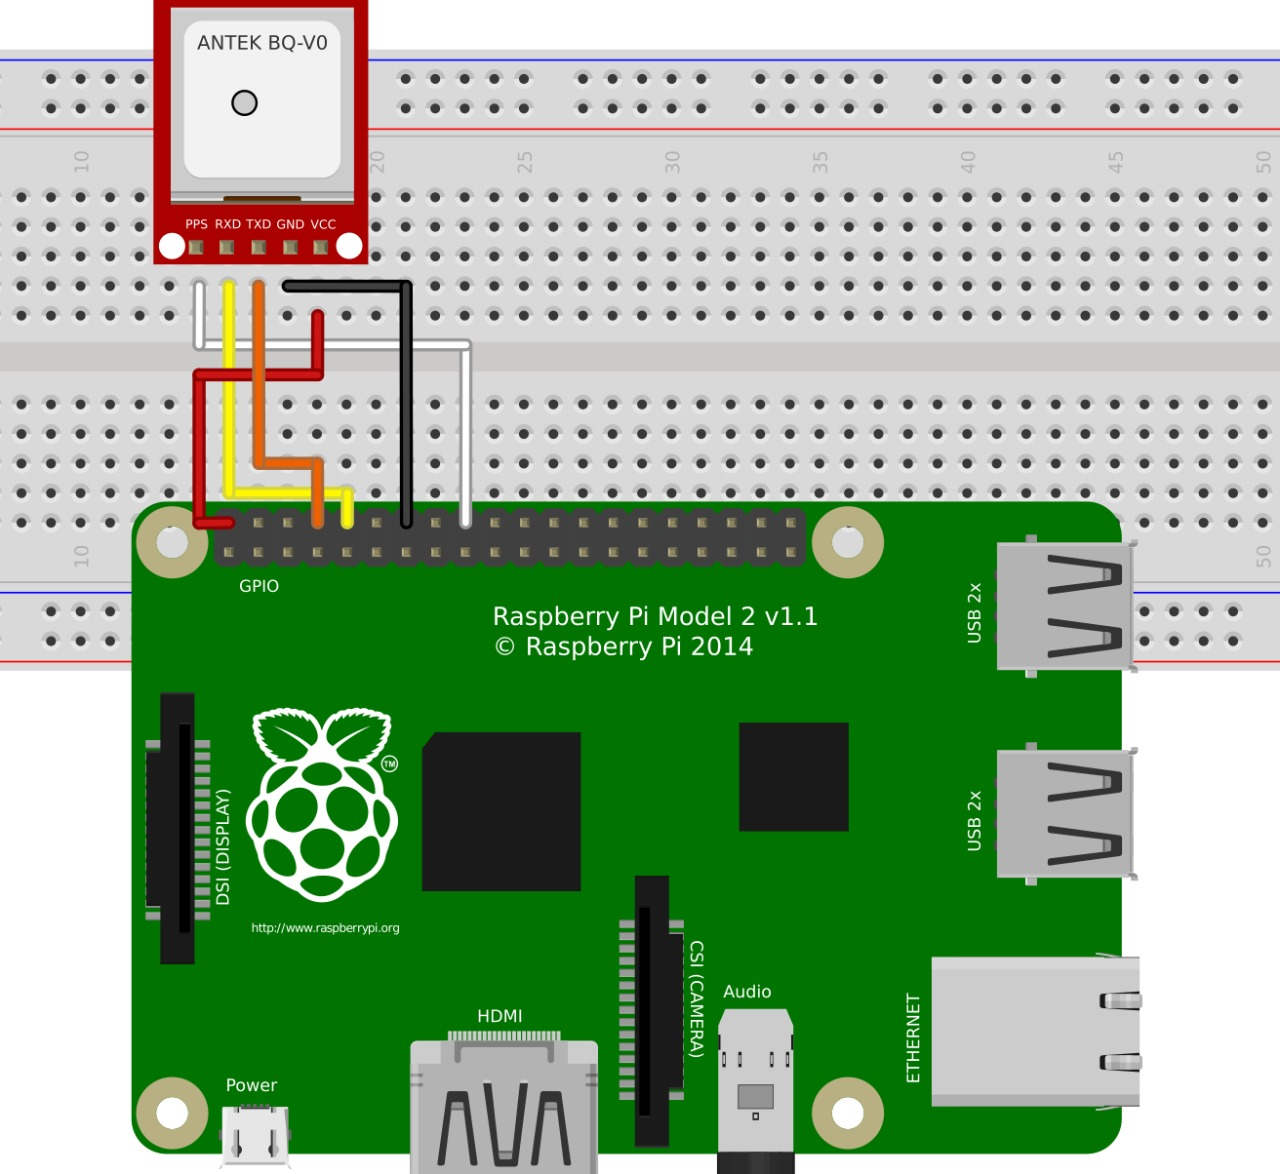
\includegraphics[width=.7\textwidth]{fig1.jpg}
\caption{ Esquema de ligação do módulo GPS com o Raspberry Pi}
\label{fig:exampleFig1}
\end{figure}
No tutorial do Anexo 1 foram feitos os seguintes passos: 
\begin{itemize}
\item Conexão do GPS no Raspberry Pi;
\item Atualização do Raspberry Pi;
\item Configurações no Raspberry Pi;
\item Instalação e conexão do GPS e PPS;
\item Instalação do NTP;
\item Configuração do NTP.
\end{itemize}
Após esse último passo o servidor NTP foi concluído com exito.
\section{Resultados e Discussões}

Durante a sua configuração, o módulo GPS enfrentou problemas de conexão com o satélite quando posicionado em locais muito fechados ou quando o céu esteve nublado. Após configurado o GPS, foi possível se obter dados referentes a: latitude, longitude, altitude e velocidade do dispositivo, assim como a hora.

Após a configuração do servidor NTP foi possível obter tanto o sinal do GPS quanto do PPS, assim como detalhes sobre a rede e parâmetros que precisam ser monitorados em tempo real para garantir a integridade do servidor, deixando pronto o servidor NTP como Stratum 1.

O servidor NTP é largamente usado para manter o tempo nos computadores e dispositivos que são conectados em uma rede. Isso permitiu com que o Raspberry Pi trabalhasse como um computador comum sem precisar de um clock físico. Porém como mostra \cite{corcoran} é possível fazer outras aplicações como, por exemplo, a sincronização de áudio em um estádio de futebol.


\section{Conclusão}\label{sec:figs}

O servidor NTP foi implementado configurado como Stratum 1 e pode ser usado em rede local através do IP do Raspberry. Foi possível observar os pontos fortes e fracos dos objetos trabalhados nesse projeto. Por tanto os objetivos do trabalho foram alcançados. 

\section{Anexos}
\subsection{link para o tutorial}
https://github.com/pedroemerick/NT-Pi
\bibliographystyle{sbc}
\bibliography{sbc-template}

\end{document}
